\documentclass{jsarticle}
\usepackage{natbib,times,plext,okumacro,url}
\usepackage{graphicx,wrapfig}
\usepackage[greek,english]{babel}
\usepackage{teubner}
\usepackage[T1]{fontenc}
\usepackage{textcomp}
\usepackage[utf8]{inputenc}


\author{授業用資料:江口聡}
%\date{4月16日}
\title{ソクラテス、プラトン}
\begin{document}
\maketitle

\section{「正しい」}

\begin{enumerate}

\item 西洋哲学の歴史のなかでは、
「正しい」と「よい」は(とりあえず)別の観念なので注意すること!
  
\item 善い、良い good ⇔ 悪い bad

\item 正しい right ⇔ 不正である wrong 
\item 正義にかなった just  ⇔ 正義に反した/不正な unjust

\item good - better - best 、 bad - worse - worst。
でもrightやjustやwrongには比較級はないぞ。(日本語では「より正しい」がある)

\item 「正しい」「不正な」は、一般には「なにかある\underline{基準}に即しているかどうか」によって判断されると主張されることがある。(しかしこれ自体が哲学的分析の対象。)

\item 哲学史・倫理学史を研究する上ではさらに翻訳の問題もある。
次のギリシア語はとりあえず暗記しておこう。(ギリシア文字は書けるように
なっておいた方がかっこいい)

 \begin{enumerate}
 \item ディカイオシュネー(正義) \textgreek{dikaios\ua{}nh} 
 \item アレテー(徳、卓越性) \textgreek{\as{}ret\ha{}} 
 \item アガトス(よい、善) \textgreek{\as{}gajos} 
 \item カロス(美、よい) \textgreek{kal{\oa}s}
 \item カコス(悪) \textgreek{kak\oa{}s} 
 \item ノモス(慣習、法律)\textgreek{n{\oa}mos} 
 \item ピュシス(自然) \textgreek{f{\ua}sis}
 \end{enumerate}




\end{enumerate}

\section{ソフィストと相対主義}


\begin{itemize}


\item 古代ギリシアの都市国家ポリス。紀元前10世紀ごろから成立。
\item 紀元前5世紀のはじめのアテネでの民主政治の発展。アテネはギリシア同盟の宗主としてペルシア戦争に勝利。

\item 民主制のもとで成功するためには、集会や法廷で弁論によって人々を説得する能力が必要だった。

\item ソフィスト sophist (智恵ある人)。職業的教師。弁論術(説得術)を教える。

\item 道徳に対する相対主義的傾向。
\item プロタゴラス「人間は万物の尺度である。在るものについては、それが在るということの。在らぬものについては、それが在らぬということの。」

\item 歴史家ヘロドトスが、社会間での風俗習慣の大きな相違を報告。

\begin{quotation}
  \small あらゆる点から見て、カンビュセス(ペルシアの王)の精神が極度に錯乱していたことは明白であると私は考える。さもなくば、いやしくも信仰や慣習に関わることを敢えて嘲笑するようなことをしたはずがないからである。実際どこの国の人間にでも、世界中の慣習の中から最も良いものを選べといえば、熟慮の末誰もが自国の慣習を選ぶに相違ない。このようにどこの国の人間でも、自国の慣習を格段にすぐれたものと考えるのである。これほど大切なものを嘲笑の種にするということは、狂人でもなければ考えられる行為といえるであろう。

  どこの国の人間でも、慣習についてこのように考えていることは、いろいろな証拠によって推論することができるが、中でも次に記すことはそのよい例といえよう。ダレイオス王がその治世中、側近のギリシア人を呼んで、どれほどの金を貰ったら、死んだ父親の肉を食う気になるか、と尋ねたことがあった。ギリシア人は、どれほどの金を貰っても、そのようなことはせぬと言った。するとダレイオスは、今度はカッラティアイ人と呼ばれ両親の肉を食う習慣を持つインドの部族を呼び、先のギリシア人を立ち会わせ、通訳を通じて彼らにも対話の内容が理解できるようにしておいて、どれほどの金を貰えば死んだ父親を火葬にすることを承知するか、とそのインド人に訊ねた。するとカッラティアイ人たちは大声をあげて、王に口を慎しんで貰いたいといった。慣習の力はこのようなもので、私にはピンダロスが「慣習こそ万象の王」と歌ったのは正しいと思われる。(ヘロドトス『歴史』紀元前5世紀)
\end{quotation}


\item → ノモスとピュシスの区別。

\item 保守的ソフィスト→ 社会の決め事(ノモス)に従うことがその社会の成
  員にとってまさに正しいことである。社会の成立と維持のため、社会の成員
  がノモスを遵守することが重要。

\item 急進的ソフィスト → 本当に「正しい」ことは存在しない。ノモス上の
  正義と道徳は、社会の支配者グループによって作られた規則にすぎない。ノ
  モスではなく、ピュシスにしたがい自分の利益を追求することこそ本当の意
  味で「正しい」。


  \begin{quote}
    アンティポン「つまり、正義とは自分が住んでいる国の決まり(ノモス)
    を犯さないということである。したがって、人間は、目撃者のいる場では
    法(ノモス)を大いに尊重し、目撃者がいない自分一人だけの場では、自
    然(ピュシス)のそれを尊重するようにすれば、正義を最も自分のために
    なるように活用することになろう。なぜなら、法の上の事柄は後に勝手に
    定められたものであるが、自然的な事柄は、変更できない必然的なものだ
    からである。」\citep[p.9]{西洋倫理思想の形成1}
  \end{quote}


\end{itemize}


 \begin{wrapfigure}{r}{50mm}
   \begin{center}
     \includegraphics[width=40mm]{image/Sculpture_of_Socrates.eps}
     \caption{ソクラテス}
   \end{center}
 \end{wrapfigure}


\section{ソクラテス}


\begin{itemize}


\item ソクラテス(469?-399 B.C.)。399 B.C.、若者たちを堕落させ、新しい鬼神の類いを祭っているという理由で裁判にかけられ有罪となり死刑。

\item プラトン(427-347 B.C.)、クセノフォン(434?-355? B.C.)、アリストファネス(448?-385? B.C.)などがソクラテスの言行を記録。

\item 無知の知。「汝自身を知れ」。助産術。問答法。エイロネイア(皮肉、空とぼけ)。

\item 知識・常識の吟味。大多数の人々に支持されているからといって、真実であるとは
限らない。

\item 「徳」の追求。「敬虔とは何か」「勇気とは何か」と定義を求める。


\item アテネの馬アブ。
  \begin{quote}
     ここに一匹の馬があるとして、それは素性のよい大きな馬なのですが、大きいために、かえって普通よりにぶいところがあって、目をさましているのには、何かアブのようなものが必要だという、そういう場合に当たるのです。つまり神は、わたしをちょうどそのアブのようなものとして、このポリスに付着させたのではないかと、わたしには思われる。つまりわたしは、あなたがたを目ざめさせるのに、各人一人一人に、どこへでもついて行って、膝をまじえて、全日、説得したり、非難したりすることを、少しもやめないものなのです。(30E\footnote{数字とabcdは、プラトンの校本や訳書で共通に使われているページ番号。最古の活字本ステファヌス版プラトン全集H. Stephanus, \emph{Platonis opera quae extant omnia}, 1578のページ数と各ページ内のABCDEという段落づけに対応する。})
  \end{quote}


\item 「吟味されない生は生きるに値しない」(『弁明』、38A))

  \begin{quote}
    人間にとっては、徳その他のことについて、毎日談論するという、このことが、まさに最大の善きことなのであって、わたしがそれらについて、問答しながら、自分と他人を吟味しているのを、諸君は聞かれているわけであるが、これに反して、吟味のない生活は、人間の生きる生活ではないと、こう言っても、わたしがこう言うのを、諸君はなおさら信じないであろう。しかしそのことは、まさにわたしの言うとおりなのだ、諸君。ただそれを信じさせることが、用意ではないのです。(38A)
  \end{quote}


  \begin{quote}
     わたしとは、どんな人間であるかといえば、もしわたしの言っていることに何か間違いでもあれば、こころよく反駁を受けるし、他方また、ひとの言っていることに何か本当でない点があれば、よろこんで反駁するような、とはいっても、反駁を受けることが、反駁することに比べて、少しも不愉快にならないような、そういう人間なのです。なぜなら、反駁を受けることの方が、より大きな善であるとわたしは考えているからです。(『ゴルギアス』 458A )
  \end{quote}

\item 「大切にしなければならないのは、ただ生きるということではなくて、善く生きるということなのだ。」(『クリトン』、48b)

\item 徳は知(エピステーメー)である。誰も進んで誤ったことはしない。

\item 子どもに、その子どもにとって善いものを与えることと、子どもが欲するものを与えることはまったく違う。→ 「善い」ことは「本人が欲すること」とは違う。(『リュシス』207D〜)

\item 399 B. C.、ソクラテスは神への不敬と若者を惑わした罪によってアテネの民会で死刑を宣告され、友人のクリトンは脱獄を勧める。

\end{itemize}


\section{プラトン『ゴルギアス』}
\begin{itemize}
\item ソクラテスの死後間もなく書かれたと推定されている。

\item ソフィストの相対主義。「ピュシス(自然)」と「ノモス(法律・慣習」の区別。

\item ソクラテスが、ゴルギアスとその弟子ポロスらの「弁論術は利益になる技術であり、ひとに力を与える」という主張を吟味し反駁。

\item ゴルギアスによれば、最高善は自由。自由であるためには他の人々を支配することができねばならず、そうするための説得の技術が弁論術。

  \begin{enumerate}
  \item 弁論術は物事の正・不正について人々を説得する技術である。
  \item 弁論術を修得したものは自分が専門の知識をもたなくても、どんなことがらについても自分の考えに従わせ専門家に打ち勝つことができる。
  \item したがって弁論術は修得者に特別な力を与え、利益を約束する。
  \item 弁論術は不正な目的にも使用できるが、弁論術そのものは道徳的に中立であり責めを負わせられるには値しない。
  \end{enumerate}


\item ソクラテス
  \begin{enumerate}
  \item 弁論術は正・不正についての真の知識を教えずむしろ根拠なく信じさせることによって人を説得するにすぎない。
  \item それゆえ弁論術はものごとの正・不正に無知なひとのあいだで彼らをだますことによって力をもつにすぎない。
  \item それゆえ弁論術は人を優れた正しい人にするには役に立たず、真の技術ではなく、技術を模倣した阿諛追従の術にすぎない。
  \end{enumerate}

\item ポロス
  は権力の獲得ことが重要であると主張。

%   \begin{enumerate}
%   \item 他人から不正を受ける方が他人に不正を加えるよりも自分にとって有害である。
%   \item 不正を犯して罰される者は、最も惨めであり、罰せられずに不正をなす者は最も幸福である。
%   \end{enumerate}

\item ソクラテスは「不正を行なうことは、不正を行なわれることより
  そのひとにとって悪いことである」「不正を行なうものは不正を行なわれる
  者より悲惨である」と主張。

%   \begin{enumerate}
%   \item 他人に不正を加える方が「より醜い」。
%   \item しかし「醜い」とは「苦しい」か「有害」かどちらかの意味である。他人に不正を加える方が「より苦しい」とは言えない。
%   \item それゆえ他人に不正を加える方が「より有害」
%   \end{enumerate}


\item 最後に登場するカリクレスは、ゴルギアスとポロスがソクラテスに説得
  されてしまったのは、周りの人びとの目を気にして、善や正義といった考え
  に過剰に譲歩してしまったからだと主張。

\item カリクレスによれば、「優れている」とは「より強い」を意味する。
  「よい」生活とは、欲望のままに生き、できるかぎり快楽をもたらす生活。

\item ソクラテス。節制し正しく生きることがよく生きること。

\item われわれは「悪い快楽」などを考えることができるのだから、
「善い」「悪い」と「快い」「苦しい」は同義ではありえない。

\item 際限のない欲望を満足させることはできない。


\end{itemize}

%  \begin{wrapfigure}{r}{50mm}
%    \begin{center}
%      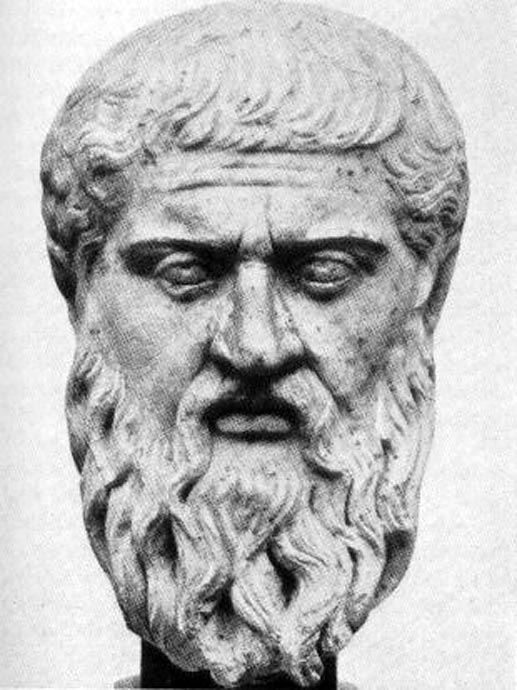
\includegraphics[width=40mm]{image/Plato.eps}
%      \caption{プラトン }
%    \end{center}
%  \end{wrapfigure}


\section{プラトン『国家』}



\begin{itemize}

\item プラトン『国家』。「正義について」の副題。

 \item プラトン『国家』でのトラシュマコスとソクラテスの対話。

\item 『ゴルギアス』でカリクレスが提出した「ピュシス」と「ノモス」の対
  比が『国家』の登場人物トラシュマコスの口を借りてくりかえされる。

\item トラシュマコス「ノモスの上での正義と道徳は、社会の支配者グループによって作られた規則、つまり、自分たち以外のすべての人びとを抑圧し、支配者自身の利益を増進させるまえに作られた規則によってなりたっている。したがって、ノモス上の正義などに騙されず、首尾よくやりとげられるときにはいつでも正義を無視してかまわないし、他人の利益ではなく自分の利益を追究せよ。唯一の合理的で自然的な正義は私利の追求である。「倫理(正義)は強者によって弱者に押しつけられるもの」

\item ソクラテス「支配者は、支配者としては、自分の利益を考えず、むしろ支配される者の利益を考える」

\item プラトン『国家』第一編でも、トラシュマコスが『ゴルギアス』でのカ
  リクレスと同様の主張を行なう。

\item トラシュマコス「倫理(正義)は強者によって弱者に押しつけられるもの」「正義とは強者の利益になることを行なうこと」「不正とは自己の利益になること」

\item ソクラテス「強者」とは「人を支配する者」。


% \item しかし支配する者が支配する者であるのは、支配する技術(\textgreek{t{\ea}qnh}をもっているから。
\item しかし支配する者が支配する者であるのは、支配する技術をもっているから。


\item しかし技術はそれを行使される人々の利益のために実行されねばならない。

\item したがって、支配者は支配される者の利益を図るべきである。

\item それゆえ正義とは強者の利益になることだということはナンセンス。

\item ソクラテス「不正」が「正義」よりも自己自身の利益になることはありえない。



\item 『国家』でのグラウコンの問題提起。われわれがうまくやりとげられるのであれば、トラシュマコスによって弁護されている生き方が最善である。


\item 「ギュゲスの指輪。」もし姿が見えなくなる指輪を手に入れれば、誰でも不正を行なうのではないか。


\item しかし現状では、もしわたしが自分の利益を追究し、他人の利益をまったく無視し、場合によっては他人に危害を加えならば、他人はわたしに対しておなじようにふるまうことになろうだろうから、結局わたし自身が損害を被ることになりかねない。そこで、ひとびとは、他のひとびとが同様にさしひかえるという条件で、各人ができるかぎり他人に危害を加えることをひかえようという相互理解に足する。「正義」は約束事であるノモス。


\item ソクラテスはこれらの立場を論駁しようと試みる。

\item 『国家』での国家の三分説と魂の三分説。

\item 国家→物質的必需品を生産する労働者、国家を防衛する軍人、国家の社会生活を組織する支配者。

\item 魂の内部で葛藤があることから、魂の中に部分があることがわかる。

\item (喉が乾いているので)あるひとが水を飲みたいと思い、また、(水が不潔なのではないかと疑って)水を飲みたくないと思う、ということから、プラトンは魂には部分があると推論。

\item ←ピタゴラス派からひきついだ魂と身体の二分説。

\item 個人→欲求的部分、気慨的部分、理性的部分

\item 正しい人生は不正な人生より幸福である。

\item (1)不正なひとは自分のさまざまな欲望をなにも制限しないので彼の欲望には限度がない。しかし欲望を満しつづけることはできないので、彼は常に不満であり不幸である。

\item (2)哲学者がだけが理性の快楽と無制限な欲望や官能の快楽を比較することができる。欲望の支配下にある人間は、自分自身がもっている種類の快楽しか知らず、より高度な種類の快楽の価値を評価できない。

\item (3)知性の快楽は純粋である。一方、欲求をもったひとが快楽とみなすものは、たいてい苦痛や不快の中止にすぎず、知識人(哲学者)が楽しみむのにくらべて本当ではない。幻想にもとづいた快楽はほんとうの快楽ではない。


\item ホッブズ(1588-1679)の利己的存在としての人間観と自然状態。

\end{itemize}



\section{プラトンの答}

\begin{itemize}

\item 国家と人間のアナロジー(434d-445e)。理性、気概、欲望の三分説。守護者(治世者)、補助者(兵士)、経済生産にたずさわる者。
\item ピュシスとノモスの対立を否定。ノモス的正義は人間本性に根ざしている。
\item ノモス的正義と個人の利益との対立も否定。ノモス的正義に合致した生活は
それ自体もっとも幸福で価値のある生活。

\item 正義は人間のピュシスに根ざしているので、正義にかなった生活を生き
  ることには客観的な価値がある。


\item 第9巻(576b以下)の議論が重要。

\item 不正な独裁者は、その欲望が満たされているときには幸福に見えるが、実際にはその欲望に隷属してしまっている。

\item 人格の三つの部分(理性、気概、欲望)はそれぞれ対応する快楽を持つ。この三通りの解釈の評価は、理性によるはずである。理性の支配下にあるひとは知識と合理性をもっているが、欲望の支配下にある人は自分がもっている種類の快楽しか知らず、より高度な種類の快楽しか評価できない。

\item 自然的世界は実はほんとうの意味では実在とは言えない。したがって、自然的世界での身体的快楽、食物や性の快楽は、実在的な快楽ではない。唯一の真実の快楽は理性の快楽。← 「イデア論」。





\end{itemize}







\nocite{田中美知太郎57:ソクラテス}
\nocite{中公世界の名著:プラトン1}
\nocite{プラトン57:ゴルギアス}
\nocite{プラトン64:ソクラテスの弁明クリトン}
\nocite{プラトン田中66:国家}
\nocite{プラトン藤沢66:ゴルギアス}
\nocite{納富信留06:ソフィスト}


\section{読書ガイド}

プラトンは読みやすいのでぜひ直接に読みたい。
江口のおすすめは『ソクラテスの弁明・クリトン』『ゴルギアス』『パイドン』
『饗宴』。『国家』は長くて読みにくいだろう。



ソクラテス・プラトンまわりは文庫や新書でよい概説書が手に入る。
特に田中美知太郎は昭和時代のプラトン研究の権威で、どの本も哲学入門として読んで
おもしろい。最近出た\cite{納富信留06:ソフィスト}がおもしろかった。

日本語で読める倫理学史については\citet{norman98:_moral_philos}が現在のベスト。
以前は\citet{macintyre67:_short_histor_of_ethic}がよいと言われていた。


\nocite{田中美知太郎57:ソクラテス}
\nocite{田中美知太郎76:ソフィスト}





\end{document}




%%% Local Variables:
%%% mode: japanese-latex
%%% TeX-master: t
%%% End:
